\documentclass{article} % For LaTeX2e
\usepackage[final]{../colm2025_conference}

\usepackage{microtype}
\usepackage{hyperref}
\usepackage{url}
\usepackage{amsthm}
\usepackage{amsmath}
\usepackage{amssymb}
\usepackage{pifont}% http://ctan.org/pkg/pifont
\usepackage{booktabs}
\usepackage{soul}
\usepackage{cancel}
\usepackage{algorithm}
\usepackage{algpseudocode}
\usepackage{graphicx}
\usepackage{subfig}
\usepackage{tablefootnote}
\usepackage{multicol}
\theoremstyle{definition}
\newtheorem{theorem}{Theorem}[section]
% \newtheorem{proof}{Proof}[section]

\usepackage{lineno}
\newcommand{\cmark}{\ding{51}}%
\newcommand{\xmark}{\ding{55}}%

\definecolor{darkblue}{rgb}{0, 0, 0.5}
\hypersetup{colorlinks=true, citecolor=darkblue, linkcolor=darkblue, urlcolor=darkblue}


\title{Week 10: Deep Dive into RLVR with nano-aha-moment}

\author{\textbf{BEH} Chuen Yang}

\newcommand{\fix}{\marginpar{FIX}}
\newcommand{\new}{\marginpar{NEW}}

\begin{document}

\ifcolmsubmission
\linenumbers
\fi

\maketitle
% Starting from this week, we are going to learn the most fun part of this project - conducting RL on LLM by yourselves! Note that you will need a GPU to do this, and if you encounter any difficulty please feel free to DM me (asap) and we will see how to solve the compute resource issue. I would expect the experiment to be run on a single GPU.
% - Step 0: Dive into this notebook deeply, and understand its content: https://github.com/McGill-NLP/nano-aha-moment/blob/main/nano_r1.ipynb
%     - Basically it applies GRPO, the RL algorithm used in DeepSeek-R1, to train a Qwen model on a task called countdown.
% - Step 1: Run the code and get some preliminary experiment results.
%     - Note: Instead of using 3B model, try 0.5B model first (so you do not need a GPU with large vRAM)
% - Step 2: Now, we will do the most challenging part in this project (so far).
%     - Adapt the code to train on the task of GSM8K - a grade school level math problem dataset.
%         - You can train qwen2.5-0.5b model first, scale up if your compute allows
%         - Dataset available here: https://huggingface.co/datasets/axon-rl/GSM-8k
%         - You need to change PROMPT_TEMPLATE accordingly because now we are dealing with another task (solving the math problem)
%         - You also need to change equation_reward_func because now we have different ways to grade the answer correctness: you can simply use string matching (because GSM8K data’s answer is simple) or you can use a more general grader (https://github.com/huggingface/Math-Verify)
% - Step 3: Write a report to summarize: the problem formulation, the method you take (GRPO’s equation, how to do the RL process), and the results you obtained.
%         - Suggestion: finish step 0-1 in one week and step 2-3 in another.
% - Final note: this assignment will take a 25% score in total as a combined assignment of week 10 - 11.

% General structure:
% - Introduction to nano-aha-moment
% - GRPO
%   - Background: DeepSeek-R1 
%   - GRPO in nano-aha-moment
% - Experiments
%   - Countdown Task (0.5B)
%   - Countdown Task (1.5B)
%   - GSM8K Task (1.5B)
% - Results & Discussion
% - Conclusion
% - Appendix A: Hyperparameters

% If you run this on the GSM8K dataset, you will see that some numbers are malformed...
%SELECT 
%     problem,
%     answer,
%     answer[1] AS first_answer_element
% FROM 
%     train
% WHERE 
%     NOT regexp_matches(answer[1], '^[0-9]+$')
% LIMIT 10;

\begin{abstract}
    This report explores the use of RLVR for base model post-training in two parts.
    Firstly, we explore how RLVR is implemented in the nano-aha-moment repository, and see it in action
    on a simple task called countdown.
    Secondly, we adapt the code to train on the GSM8K dataset, a grade school level math problem dataset.
    We detail any insights and challenges encountered during the process,
    and present the results of our experiments.
\end{abstract}

\section{Motivation}

Much like how pre-training looks deceptively easy (\cite{beh-2025-b}),
reinforcement learning with verifiable rewards (RLVR) is another algorithm
which promises amazing reasoning capabilities just by training a model to do 
math/computing/logic problems (which lend themselves VERY well to uncomplicated verification mechanisms) 
(\cite{grpo, r1, tulu3}).

Indeed, as with pre-training (\cite{beh-2025-b}), this overly-simplistic perspective hides 
a lot of the ugly details that make RLVR work.
In this report, we will explore the nano-aha-moment (\cite{nano-aha-moment}) repository,
and in doing so, explore qualitatively how RLVR works (and doesn't) in practice.

\section{nano-aha-moment}
Apparently continuing in the nanoGPT (\cite{nanoGPT}) tradition,
the nano-aha-moment (\cite{nano-aha-moment}) repository provides a minimalistic implementation 
of RLVR (Reinforcement Learning with Verifiable Rewards) using Group Relative Policy Optimization (GRPO) (\cite{grpo}).
In particular, it follows the setup of DeepSeek-R1 and R1-Zero (\cite{r1}),
which uses GRPO with relatively simple mechanisms to train language models on reasoning tasks.

While similar minimalistic repositories for R1-style RLVR exist such as TinyZero (\cite{tinyzero}),
nano-aha-moment (\cite{nano-aha-moment}) distinguishes itself through the following means \footnote{
    Unfortunately the repository itself is not updated with robust quality checks,
    which resulted in a few headscratchers before experiments could be run.
    We detail some of these issues in Appendix \ref{sec:nano-aha-moment-issues}.
}:
\begin{itemize}
    \item It does not offload the RLVR algorithm implementation to complex libraries such as veRL (\cite{veRL, veRL2})
and HuggingFace's trl (\cite{trl}), instead implementing the GRPO algorithm directly in PyTorch. 
    \item It has a small codebase ($\sim$ 1.5k lines of decently-commented code), which 
        makes it easy to understand how RLVR with GRPO works.
    \item It is designed to be run on a single GPU.
    \item As with nanoGPT (\cite{nanoGPT}), WandB \cite{wandb} integration for convenient logging.
\end{itemize} 

These features make it a good analogue to nanoGPT (\cite{nanoGPT}) for RLVR using GRPO,
serving as a pedagogical tool for understanding RLVR concepts, 
as well as for experimenting with RLVR on (very) small language models.

\subsection{Training Loop}

Unlike in nanoGPT (\cite{nanoGPT}), where most features have to be implemented from scratch,
\cite{nano-aha-moment} use the HuggingFace (\cite{HuggingFace}) library
for model training, inference, tokenization, and dataset loading in nano-aha-moment.
As such, perhaps the only salient feature of nano-aha-moment (\cite{nano-aha-moment})
is the training loop, which can be found in \href{../../code/nano-aha-moment/nano_r1_script.py}{here (Countdown-3-to-4)} and 
\href{../../code/nano-aha-moment/nano_r1_gsm8k.py}{here (GSM8K)}.

We defer a detailed discussion to the next section, where we first discuss the GRPO algorithm
used by \cite{nano-aha-moment}, and then provide a sketch of the training loop
used in our experiments in Algorithm \ref{alg:grpo-nano-aha-moment}.

\section{More on GRPO}

Since the RLVR algorithm implemented in nano-aha-moment (\cite{nano-aha-moment}) is based on 
R1-Zero (\cite{r1}), we will first provide a brief overview of the GRPO
algorithm (\cite{grpo}) used in R1-Zero (\cite{r1}).

\subsection{GRPO vs PPO}
Consider a policy network $\pi_\theta$ and critic network $V_\phi$ in a single-state,
single-action armed bandit environment with state $s$ and action $a = (o_1, \dots, o_n)$,
where $o_k$ is the $k$-th output token of the language model.

Both PPO and GRPO (\cite{ppo, grpo}) maximize this objective function\footnote{
    This is not PPO as used in RLHF by \cite{InstructGPT-2022}, rather the one used in RLVR by \cite{grpo}.
    Notably, the KL Divergence term is incorporated into the objective instead of the reward function.
    We show this formulation of PPO to highlight the fact that, ultimately, GRPO is just a 
    realization of PPO with a different way of computing the advantage $A(s, a)$.
}:
\begin{equation}
    \label{eq:obj-fn}
    \begin{array}{rl}
        \mathcal{J}(\theta) &= \mathbb{E}_{(s, o_1, \dots, o_n) \sim \pi_\theta} \left[ 
            \displaystyle
            \frac{1}{n} \sum_{k = 0}^n \min \left\{
                \frac{\pi_\theta(o_k|s, o_{< k})}{\pi_{\theta_{old}}(o_k|s, o_{< k})} A(s, a),
                g(s, a)
            \right\}
        \right] {\displaystyle - \lambda D_{KL}(\pi_\theta || \pi_{\theta_{old}})} \\
    \end{array}
\end{equation}
where ${\displaystyle g(s, a) = clip\left(\frac{\pi_\theta(o_k|s, o_{< k})}{\pi_{\theta_{old}}(o_k|s, o_{< k})}, 1 - \epsilon, 1 + \epsilon \right) A(s, a)}$,
and $\pi_{\theta_{old}}$ is the policy network from the previous GRPO step.


However, where in PPO with Generalized Advantage Estimation (GAE) (\cite{ppo, gae}), $A(s, a) = r(s, a) - V_\phi(s)$ is the one-step advantage of the action $a$ in state $s$,
in GRPO (\cite{grpo}), $A(s, a) = \frac{r(s, a) - \mu}{\sigma}$, where $\mu$ and $\sigma$ are the mean and standard deviation of the rewards for a given batch of state-action
pairs $(s_1, a_1), \dots, (s_r, a_r)$.

Note how in both cases, the advantage $A(s, a)$ is the same regardless of the output token $o_k$. This is 
because the entire output is considered a single action.

\subsection{Why GRPO?}

Where policy gradient algorithms are concerned (\cite{Weng-2018}), Proximal Policy Optimization (PPO) (\cite{ppo}) 
has been a standard choice as it contains many tricks and improvements
that serve to greatly stabilize the high-variance training process inherent to RL.
Namely, these are:
\begin{itemize}
    \item Using a value function baseline, approximated by a critic network, to reduce variance in the policy gradient
    \item Using Generalized Advantage Estimation (GAE) to compute advantages
    \item Using a clipped surrogate objective to prevent large updates to the policy
\end{itemize}

However, when hundreds of millions, or even billions, of parameters are involved,
it can become prohibitive to host the language model, let alone increase the memory footprint
by adding a separate critic network. \footnote{
    Parameter sharing between the policy and critic networks is of course possible.
    However, this results in a network that tries to optimize for two different objectives at once,
    which \textit{can} lead to suboptimal performance.
}

In order to address these compute constraints, DeepSeek proposed a new algorithm called Group Relative Policy Optimization (GRPO) (\cite{grpo}),
which is very similar to PPO (\cite{ppo}) in most respects, except that it does not require a critic network.
Instead, \cite{grpo} use batch reward statistics to estimate the relative advantage of certain actions (i.e. outputs) over others.

Conceptually speaking, this is a counterintuitive idea. GRPO (\cite{grpo}) effectively eschews a high-quality value function baseline 
in favor of an extremely local and coarse state-value estimate, which should result in destabilized training.

However, \cite{grpo} are able to deliver first-rate empirical results when used to 
train large language models, with DeepSeekMath-7B achieving better Top-1 scores on 
the MATH benchmark than models up to 10x larger, such as Qwen2-72B (\cite{Qwen2}) and WizardMath-70B (\cite{wizardmath}). \footnote{
    For some hypotheses why, see \cite{beh-2025}.
}

Coupled with the fact that GRPO (\cite{grpo}) does not require a critic network and thus
allows for reduced memory footprint, it has become a good choice for RL post-training of large language models specifically.

\subsection{GRPO in nano-aha-moment}
While we do not have access to the source code used in the training of DeepSeek-R1 (\cite{r1}),
the nano-aha-moment (\cite{nano-aha-moment}) repository does provide an implementation which appears to closely
follow the methodology described in \cite{r1}.

In fact, directly inspecting the source code reveals that the gradient $\nabla \mathcal{J}(\theta)$ is
\begin{equation}
    \label{eq:grpo-grad}
    \begin{array}{rl}
    \nabla \mathcal{J}(\theta) & = \mathbb{E}_{(s, o_1, \dots, o_n) \sim \pi_\theta} \left[ 
        \displaystyle
        \frac{1}{n} \sum_{k = 0}^n \min \left\{
            \frac{\pi_\theta(o_k|s, o_{< k})}{\pi_{\theta_{old}}(o_k|s, o_{< k})} A(s, a),
            g(s, a)
        \right\}
    \right] \\ 
    & {\displaystyle - \lambda \left[\log\left(\frac{\pi_{\theta_{ref}}(o_k|s, o_{< k})}{\pi_{\theta}(o_k|s, o_{< k})}\right) - \frac{\pi_{\theta_{ref}}(o_k|s, o_{< k})}{\pi_{\theta}(o_k|s, o_{< k})} - 1\right]}
    \end{array}
\end{equation}
where $g(s,a)$ is as in Equation \ref{eq:obj-fn}, and $\pi_{\theta_{ref}}$ is the original, 
pre-trained policy network, and the second line is an unbiased estimator of the KL divergence 
$D_{KL}(\pi_\theta || \pi_{\theta_{ref}})$ (\cite{kl-approx}).
This is almost identical to the gradient shown by \cite{grpo}, 
which strengthens our belief that nano-aha-moment (\cite{nano-aha-moment}) is 
a faithful implementation of GRPO (\cite{grpo}).

We give a sketch of the algorithm in \ref{alg:grpo-nano-aha-moment}, based on directly inspecting its source code.
This algorithm will be used in all our experiments in the next section.

\begin{algorithm}
    \caption{GRPO in \cite{nano-aha-moment}}
    \begin{algorithmic}[1]
        \State Policy network $\pi_\theta$, pre-trained policy network $\pi_{\theta_{ref}}$, 
        hyperparameters, questions $\mathcal{S}$
        \State Initialize $\theta \leftarrow \theta_{ref}$, $\theta_{old} \leftarrow \theta_{ref}$
        \While{not converged}
            \State Sample $m$ questions $\mathcal{S}_m = \{s_i\}_{i=1}^m \subseteq \mathcal{S}$
            \State Autoregressively generate $n$ answers each for $\mathcal{S}_m$, using $\pi_\theta$. Define the answers as $\mathcal{A}_{mn} = \{\alpha_{ij}\}_{i=1, j=1}^{i=m, j=n}$
            \State Compute rewards $r(s_i, \alpha_{ij})$ for each $(s_i, \alpha_{ij}) \in \mathcal{S}_m \times \mathcal{A}_{mn}$
            \State Compute batch statistics $\mu, \sigma$ for rewards $r(s_i, \alpha_{ij})$
            \State Compute advantages $A(s_i, \alpha_{ij}) = \frac{r(s_i, \alpha_{ij}) - \mu}{\sigma}$
            \State Calculate logprobs of each token $t_j$ of $\alpha_{ij}$ under $\pi_{\theta_{ref}}$
            \State Update $\theta_{old} \leftarrow \theta$
            \State Update $\theta \leftarrow \theta + \alpha \nabla \mathcal{J}(\theta)$ (Equation \ref{eq:grpo-grad})
        \EndWhile

        \hspace*{-40pt} \textbf{Output:} GRPO-trained policy $\pi_\theta$
    \end{algorithmic}

    \label{alg:grpo-nano-aha-moment}
\end{algorithm}


\section{Experiments}

As part of exploring how RLVR works, we want to test
just how good nano-aha-moment (\cite{nano-aha-moment})
is at training language models on reasoning and math tasks.

As such, we will train models on two different tasks before evaluating
their Pass@1 performance on the tasks.

\subsection{Tasks}
Both tasks were split into train and test sets, with
the test set consisting of 500 randomly selected samples from the original dataset. All other samples were used for training.

\subsubsection{Countdown-3-to-4}
Countdown-3-to-4 (\cite{countdown}) is a simple task where the model is given three or four numbers, as well as a target number,
and must yield a mathematical expression in +, -, *, / that evaluates to the target, using each number at most once.

Though conceptually this task can be generated by a simple program,
\cite{countdown} is a dataset of 490,364 such problems, all of whose answers
are programmatically verified using Python's eval function.

Although this task can be quickly solved using tree search methods,
the need (in the worst case) to exhaustively evaluate all possible expressions
means that the task should be pretty difficult for a language model to solve.
This would be less of a problem if the language model has good numerical intuition
and reasoning capabilities, but it makes the task harder in general.

\subsubsection{GSM8K}
GSM8K is a grade school level math problem dataset.
It consists of 8,792 math problems, each with a single integer answer.

The problems are designed to be solvable by a grade school student, 
and cover a wide range of topics such as arithmetic, algebra, and geometry.

Due to the natural language format, this task is a lot harder to solve algorithmically, and it tests models' ability to parse 
natural language math problems, reason about numbers, and perform arithmetic operations correctly.

\subsection{Experimental Configurations}

Due to limited compute budget, each model and task combination was only tested with one run
This also means that hyperparameters were tuned with expert advice and
a desire to balance the training epoch count and training throughput, 
rather than extensive hyperparameter sweeping.

Training was conducted on a single NVIDIA 4090 GPU with 48GB of VRAM \footnote{
    Thanks Chann.
}, and all runs took a combined $\sim$ 33 hours of wall-clock time to complete.

\begin{table}[h]
    \centering
    \begin{tabular}{|l|c|c|c|c|}
        \hline
        \textbf{Hyperparameter} & \multicolumn{2}{c|}{\textbf{Countdown-3-to-4}} & \multicolumn{2}{|c|}{\textbf{GSM8K}} \\
        \hline
        Model Family & \multicolumn{4}{c|}{Qwen2.5} \\
        \hline
        Model Scale & 0.5B & 1.5B & 0.5B & 1.5B \\
        \hline
        Batch Size & \multicolumn{4}{c|}{16} \\
        \hline
        Learning Rate & \multicolumn{4}{c|}{1e-6} \\
        \hline
        Max. Response Length & \multicolumn{4}{c|}{512} \\
        \hline
        Completions per Task & \multicolumn{4}{c|}{8} \\
        \hline
        Episodes per GRPO Iteration & 1024 & 1024 & 16 & 16\\
        \hline
        KL Divergence Coefficient $\lambda$ & \multicolumn{4}{c|}{0} \\
        \hline
    \end{tabular}
    \caption{Hyperparameters used in our experiments.}
    \label{tab:hyperparams}
\end{table}

The hyperparameters in Table \ref{tab:hyperparams} were used for both experiments.
They were mostly kept the same for parity, though they vary quite
a bit from the defaults in nano-aha-moment (\cite{nano-aha-moment}).

A notable exception is the \texttt{eps\_per\_iteration} parameter, which was set to 1024 for the countdown task,
and 16 for the GSM8K task. The \texttt{GSM8K} task has much fewer samples ($\sim$ 8k samples) than the \texttt{countdown} task ($\sim$490k), 
and thus fewer samples are required to achieve the same number of training epochs. In order to 
leverage the full computing capacity of the GPU at 1.5B scale (thus maximizing training throughput), 
we set the batch size to 16, necessitating a minimum episodes per GRPO iteration of 16.

\subsection{Reward Modelling}
As with most RL setups, the reward function design is crucial to the success of the RLVR algorithm.

In creating R1 and R1-Zero, \cite{r1} appeared for a rather simple reward function.
While the exact details of the reward function are not disclosed \footnote{
    The most probable explanation is that the reward functions 
    vary from task to task, and take too much space to document comprehensively.
}, it is said to have 2 principal components:
\begin{itemize}
    \item Format Reward: The model must pen its thoughts in between $<$think$>$ and $</think>$ tags.
    \item Accuracy Reward: The model must output the correct answer to the problem in a specified format.
    This is enforced either with rule-based methods, or with external tools like a compiler.
\end{itemize}

We speculate that these rewards allow the model's responses to be evaluated most conveniently
(hence the moniker "verifiable rewards"), and leave little room for undesirable optimizations
such as reward hacking, for example, by outputting the same answer over and over again
in hopes of getting some rewards.

This design pattern is also followed in nano-aha-moment (\cite{nano-aha-moment}),
and the reward function is solely comprised of the same two components,
with the inclusion of an additional 0.5 reward if the model outputs an answer in the correct format,
but its response is otherwise malformed (to encourage answering of questions).

For brevity, we will not include the full implementations here. They can instead
be found in \href{../../code/nano-aha-moment/nano_r1_script.py}{here (Countdown-3-to-4)} and 
\href{../../code/nano-aha-moment/nano_r1_gsm8k.py}{here (GSM8K)}.

\subsection{Evaluation}
The evaluation of the models is done using the Pass@1 metric across the entire test set.
Specifically, we measure how many of the model's answers to the test set problems
are verifiably correct, given only one attempt to answer each problem.

This is the least taxing evaluation metric, as it does not require the model to
generate multiple answers to the same problem, and is thus the most suitable for our 
(compute-constrained) experiments.

\subsection{Hypotheses}
\label{sec:hypotheses}
Before discussing the result, we want to make some hypotheses about the performance of RLVR on the two tasks,
based on what we know about the tasks and their difficulty for language models.

Despite anecdotal observations that tasks like Countdown-3-to-4 (\cite{countdown}) would 
be harder for humans to solve as compared to GSM8K, we nevertheless hypothesize
on grounds of algorithmic tractability that RLVR will perform better on Countdown-3-to-4 (\cite{countdown}) than on GSM8K.

Namely:
\begin{itemize}
    \item RLVR will increase the Pass@1 score of Countdown-3-to-4 and GSM8K tasks across the board.
    \item Countdown-3-to-4 will require fewer training epochs to achieve good performance than GSM8K.
    \item After training, Countdown-3-to-4 will be solved with a higher Pass@1 score than GSM8K.
\end{itemize}

\section{Results}

\subsection{Countdown-3-to-4}

The results of the RLVR training on the Countdown-3-to-4 task can be found in Figure \ref{fig:countdown-results}.

At the end of 1000 training steps, the Pass@1 scores of the 0.5B and 1.5B models 
are quite similar, hovering somewhere around 0.35. 

Though this appears better than random guessing, qualitative analyses of the model's 
reasoning traces reveal failures to engage in any meaningful thinking. 
Consider this excerpt from Qwen2.5-1.5B:
\begin{quote}
    \texttt{(Numbers: 17, 54, 13. Target: 50.)} \\
    \texttt{Answer: <think> I need to use the numbers 17, 54 and 13 to make the equation 50. </think>
<answer>((54) - (17) + (13))</answer><|endoftext|>}
\end{quote}
This answer is correct, but probably a fluke, as the model's reasoning trace 
simply repeats the question context, and does not engage in any meaningful reasoning.

Indeed, it uses the exact same equation for another question (which it gets wrong):
\begin{quote}
    \texttt{(Numbers: 54, 33, 31. Target: 27.)} \\
    \texttt{Answer: <think> I need to use the numbers 54, 33 and 31 to make the equation 27. </think>
    <answer>((54) - (33) + (31))</answer>}
\end{quote}

Even more egregious is Qwen2.5-0.5B, which is even more enthusiastic about using the 
same equation form for every question:
\begin{quote}
    \texttt{(Numbers: 49, 48, 40, 42. Target: 81.)} \\
    \texttt{Answer: <think> Given the numbers [49, 48, 40, 42] </think>
<answer>(49 - 40 + 48 - 42)</answer><|endoftext|>}
\end{quote}
\begin{quote}
    \texttt{(Numbers: 40, 7, 93, 2. Target: 94.)} \\
    \texttt{Answer: <think> Given the numbers [40, 7, 93, 2] </think>
    <answer>(93 - 2 + 40 - 7)</answer>}
\end{quote}
\begin{quote}
    \texttt{(Numbers: 20, 27, 96, 46. Target: 97.)} \\
    \texttt{Answer: Given the numbers [20, 27, 96, 46] </think>
    <answer>(96 - 20 + 46 - 27)</answer>}
\end{quote}


However, the 1.5B model is able to learn the task much faster,
achieving that 0.35 Pass@1 score in just 200 training steps, 
while the 0.5B model takes about 800 training steps to reach the same score.

Somewhat surprisingly, even though the 0.5B model does not experience
sustained decreases in performance, the 1.5B model's Pass@1 reaches a peak
nearing 0.4 at around 700 training steps, before slowly declining to the final score of 0.35.

\begin{figure}
    \centering
    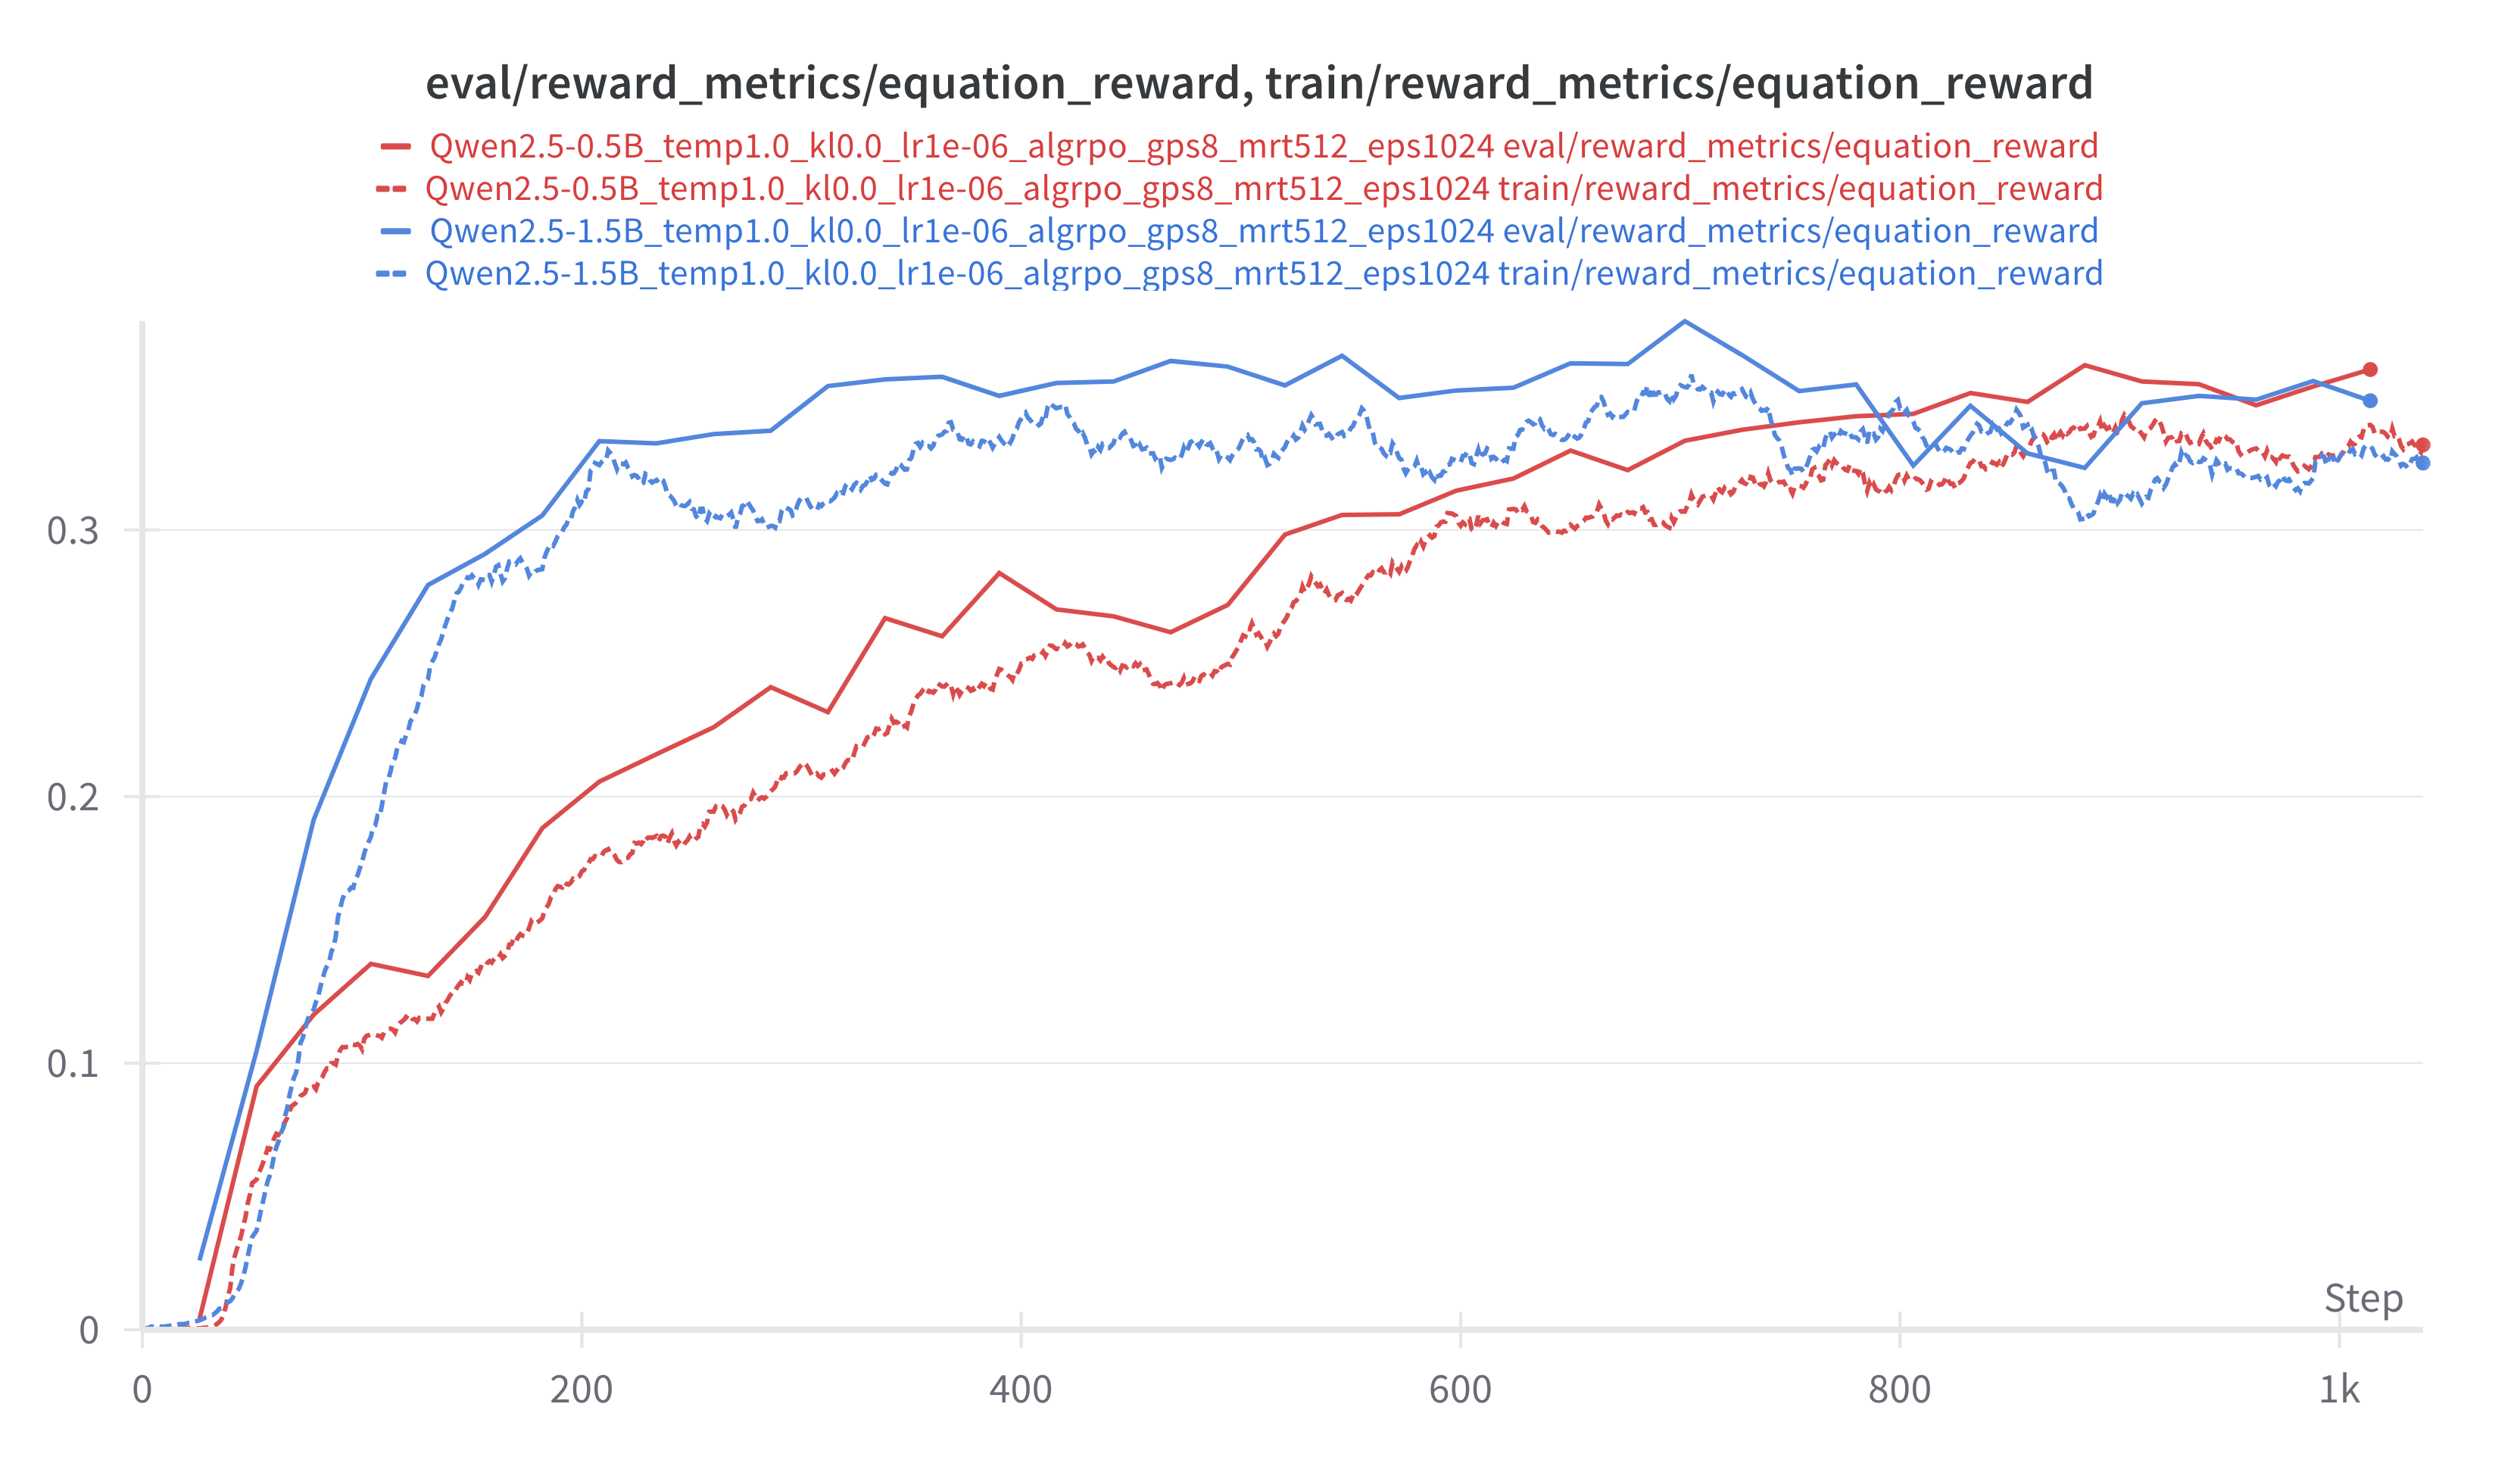
\includegraphics[width=0.8\textwidth]{images/Countdown.png}
    \caption{
        Performance of RLVR on Countdown-3-to-4 task. 
        Dotted lines are training curves,
        solid lines are Pass@1 scores on the test set.
        (Red) Qwen2.5-0.5B, (Blue) Qwen2.5-1.5B.
        Curves are smoothed using Time-Weighted Exponential Moving Average (TWEMA) with $\alpha = 0.95$.
    }
    \label{fig:countdown-results}
\end{figure} 

\subsection{GSM8K}
The results of the RLVR training on the GSM8K task can be found in Figure \ref{fig:gsm8k-results}.

Unlike on the Countdown-3-to-4 task (\cite{countdown}), the 1.5B model achieves a much higher Pass@1 score
than the 0.5B model after 1000 training steps, with the 1.5B model achieving a Pass@1 score above 0.8,
and the 0.5B model achieving a Pass@1 score of around 0.5.

Interestingly, also unlike on the Countdown-3-to-4 task (\cite{countdown}), 
both models do NOT start out with a Pass@1 score of 0.0, with both hovering rather safely
above that threshold at the start of training.

On GSM8K, both models learnt at approximately the same pace, with both experiencing
rapid increases in Pass@1 score in the first 200 training steps,
before slowly but surely converging to their respective Pass@1 scores at the final step.

Interestingly, both models are quite cogent in their reasoning traces,
with the 1.5B model producing answers such as:
\begin{quote}
    \texttt{
        Question: Mason is trying to download a 880 MB game to his phone. After downloading 310 MB, his Internet connection slows to 3 MB/minute. How many more minutes will it take him to download the game? Show your work in <think> </think> tags, and return the final answer as a single number in <answer> </answer> tags, for example <answer>5</answer>, not <answer>the answer is 5</answer>.<|im\_end|>
    } \\
    \texttt{Answer: <think>
        First, we need to determine how much of the game Mason has already downloaded, which is 310 MB.
        Then, we need to find out how much more data he needs to download, which is the total game size minus the downloaded size: 880 MB - 310 MB = 570 MB
        Now, we know that his internet connection slows down to 3 MB/minute. To find out how many more minutes it will take to download the remaining 570 MB, we divide the remaining data by the download speed: 570 MB / 3 MB/minute = 190 minutes
        So, it will take Mason an additional 190 minutes to download the game.
        </think>
        <answer>190 </answer><|endoftext|>
    }
\end{quote}

and the 0.5B model adopting a similar reasoning style:
\begin{quote}
    \texttt{(Same question as above.)} \\
    \texttt{
        Answer: <think>
         Mason has a total download of 880 MB - 310 MB = 570 MB left to download. His Internet connection slows to 3 MB/minute, so the time it will take to download the remaining 570 MB is 570 MB / 3 MB/minute = 190 minutes. </think>
<answer>190</answer><|endoftext|>
    }
\end{quote}


\begin{figure}
    \centering
    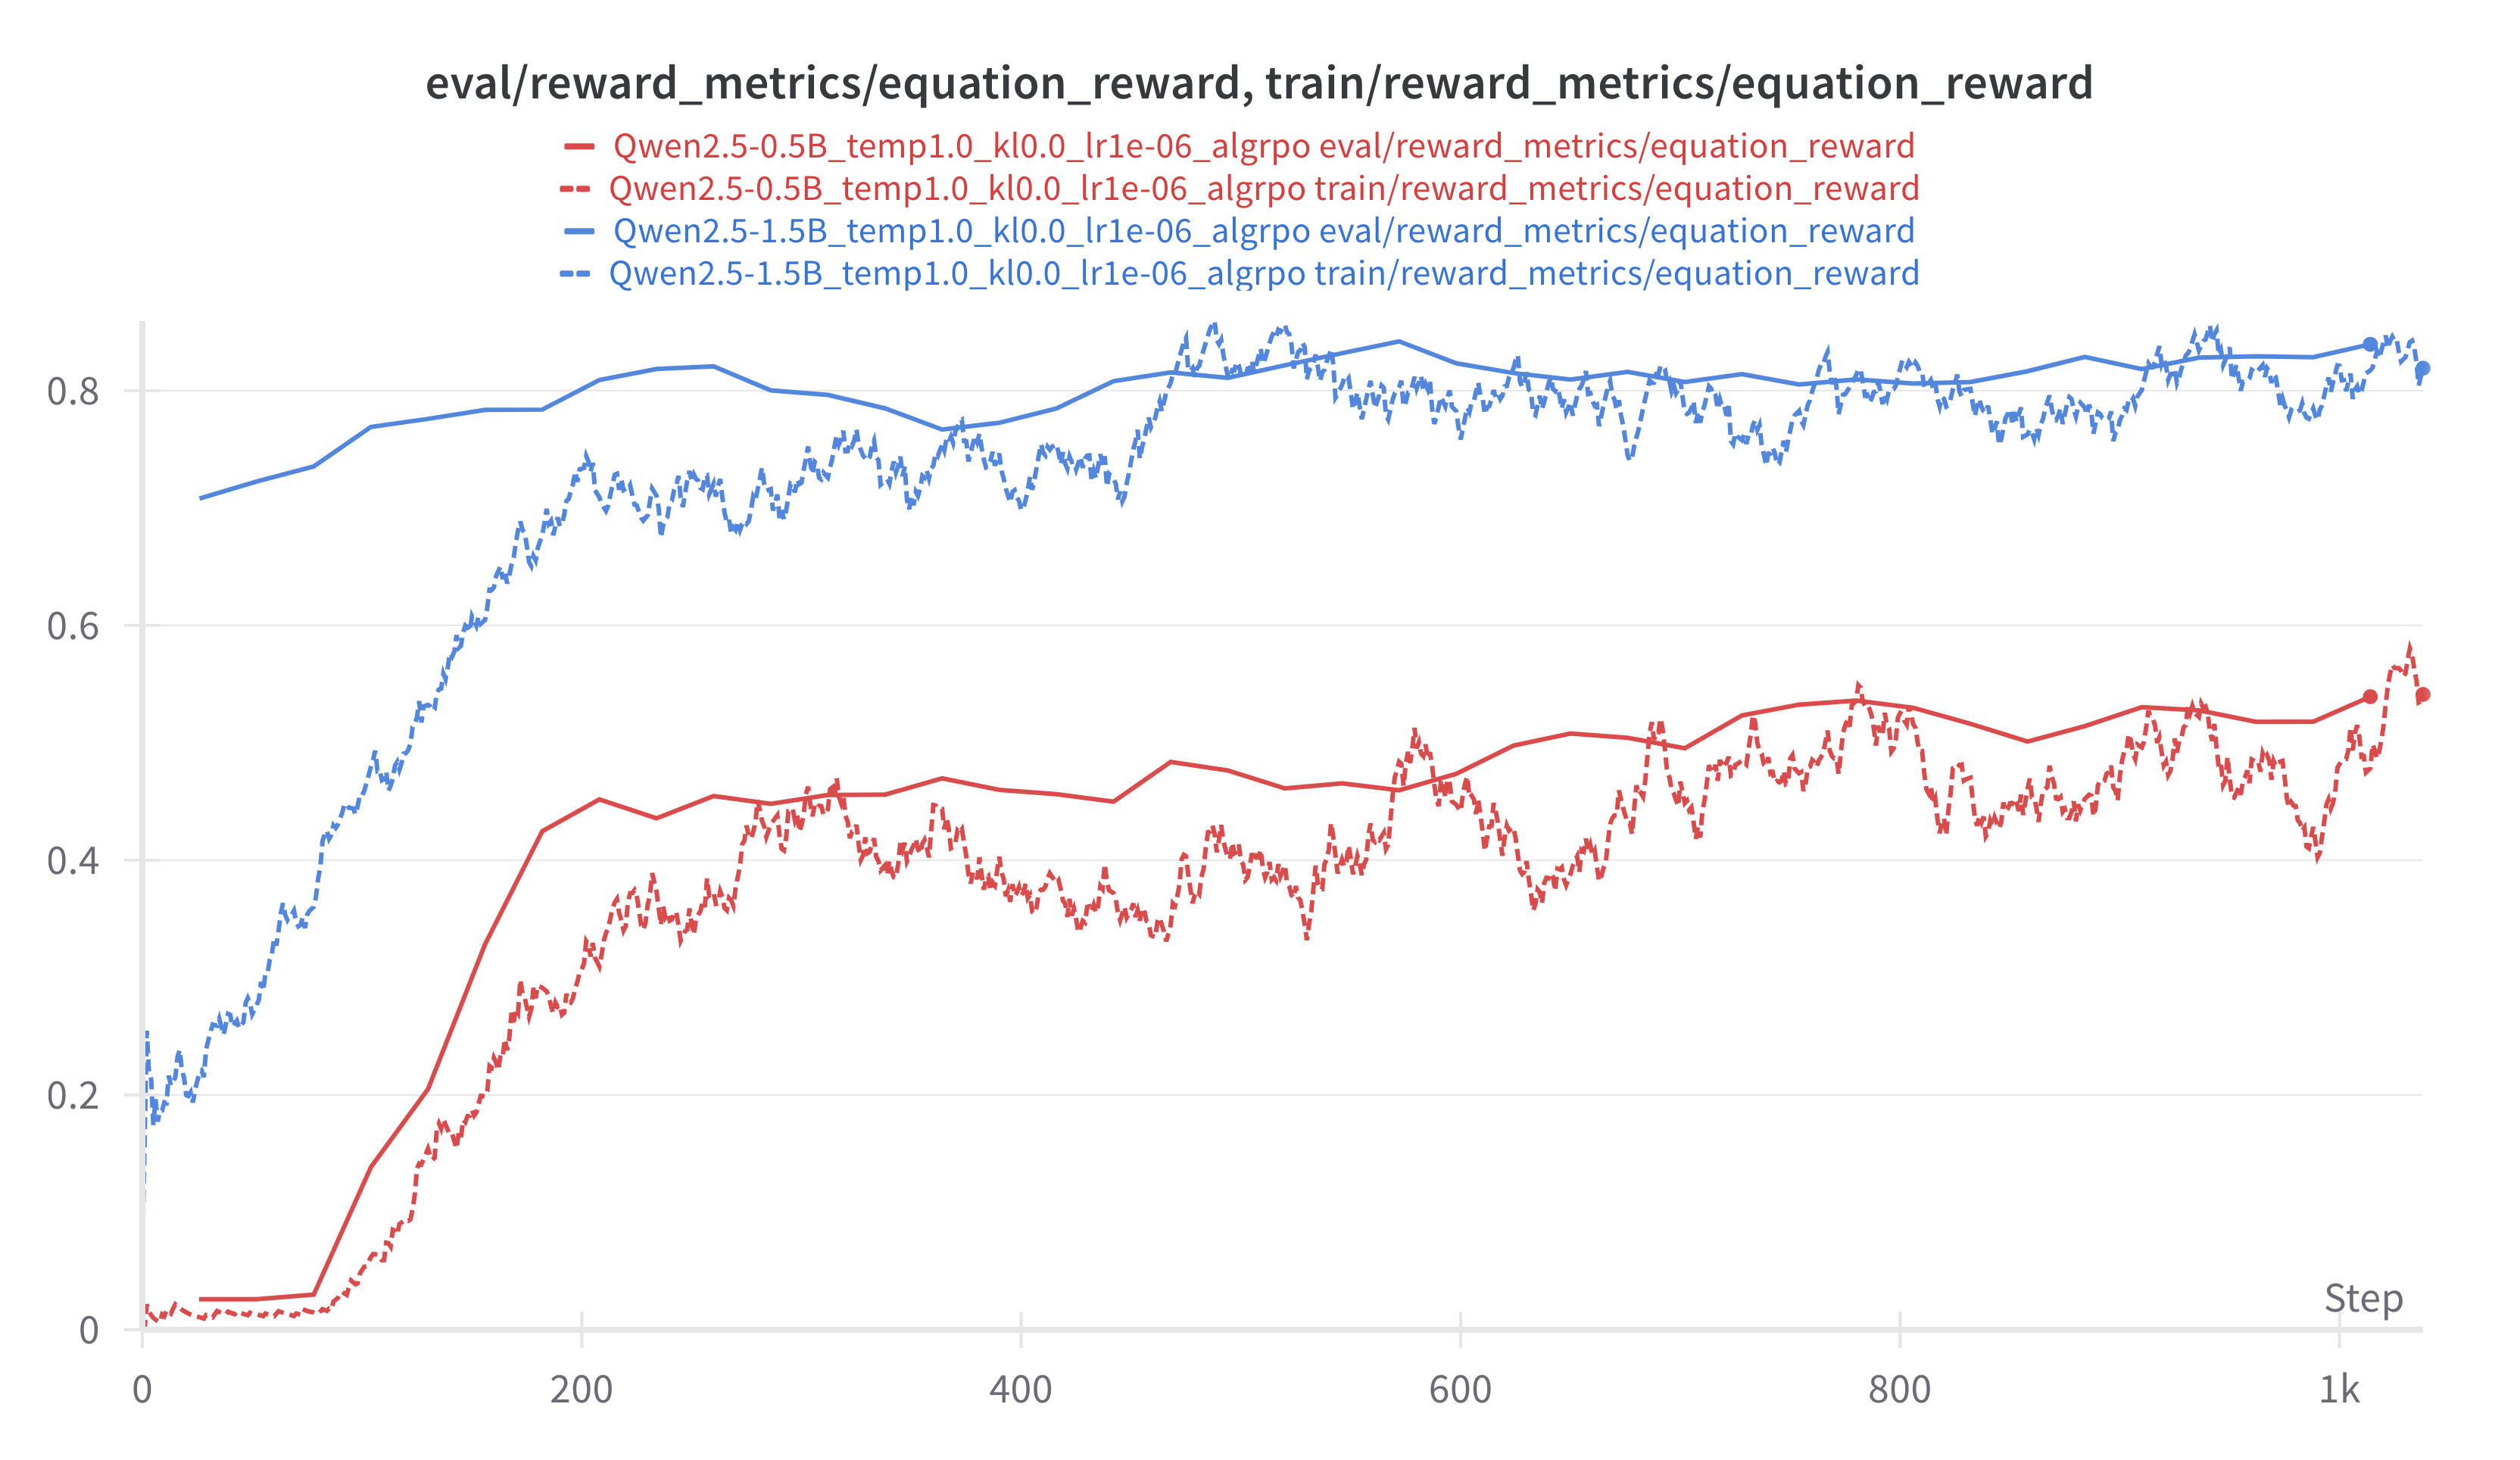
\includegraphics[width=0.8\textwidth]{images/GSM8K.png}
    \caption{
        Performance of RLVR on GSM8K task. 
        Dotted lines are training curves, 
        solid lines are Pass@1 scores on the test set.
        (Red) Qwen2.5-0.5B, (Blue) Qwen2.5-1.5B.
        Curves are smoothed using Time-Weighted Exponential Moving Average (TWEMA) with $\alpha = 0.95$.
    }
    \label{fig:gsm8k-results}
\end{figure}

\subsection{Checking Our Hypotheses}
We can now check our hypotheses from Section \ref{sec:hypotheses} against the 
results we have obtained.
\begin{itemize}
    \item RLVR will increase the Pass@1 score of Countdown-3-to-4 and GSM8K tasks across the board.
        \begin{itemize}
            \item \textbf{True.} All models end training with a better Pass@1 score than they started with.
        \end{itemize}
    \item Countdown-3-to-4 will require fewer training epochs to achieve good performance than GSM8K.
        \begin{itemize}
            \item \textbf{False.} Qwen2.5-1.5B on GSM8K achieves a Pass@1 score of 0.7 after 200 training steps,
                while all models on Countdown-3-to-4 fail to ever break the 0.5 Pass@1 score.
        \end{itemize}
    \item After training, Countdown-3-to-4 will be solved with a higher Pass@1 score than GSM8K.
        \begin{itemize}
            \item \textbf{False.} The 1.5B model on GSM8K achieves a Pass@1 score above 0.8, 
                while the 1.5B model on Countdown-3-to-4 only achieves a Pass@1 score of 0.35.
                Moreover, the 0.5B model on GSM8K achieves a Pass@1 score of 0.5, compared to 
                a similar Pass@1 score of 0.35 for the 0.5B model on Countdown-3-to-4.
        \end{itemize}
\end{itemize}
These results are overall rather surprising, and they are points of interest to consider
when reflecting on how RLVR works in practice.

\section{Discussion}
\subsection{Necessary Caveats}
Before elaborating on the results, we have to point out some limitations of our experiments,
which are primarily borne out of limited compute budget:

Firstly, our results may not be statistically significant, as each experimental configuration
was only run once. It is very plausible that our results are as good / bad as they are purely due to 
random chance, and that the true performance of RLVR on these tasks is much better / worse than what we report here.

Secondly, our results are not "optimized" in the sense that no hyperparameter sweeping
or prompt engineering was done.
Any choice of hyperparameters/prompts was made with reference to the defaults in nano-aha-moment 
(\cite{nano-aha-moment}), as well as expert consultations.
This means that our results may not be the best possible performance of RLVR on these tasks,
and that with more compute budget, we could have achieved better results.

\subsection{GSM8K May Be Easier Than Countdown-3-to-4 For LLMs}
One way to rationalise our results is that GSM8K, by nature, is a much easier task than 
Countdown-3-to-4. Rather than having to autonomously enumerate and evaluate all possible expressions
to find the correct answer, GSM8K problems often come with a lot of context and 
natural language cues that could hint to language models how they should use
mathematical techniques to solve the problem.

\subsection{Prompt Engineering May Be Required to Make RLVR Work}

We did not do any prompt engineering for the Countdown-3-to-4 task, as compared to GSM8K.

This is because we believed that the default prompt template was already optimized for the task by \cite{nano-aha-moment},
whereas there was no such default prompt for GSM8K, and we had to create one ourselves
to be as specific as possible about what we want the model to do.

Somewhat naively, this leads us to believe that performing similar prompt engineering
on the Countdown-3-to-4 task could lead to better results (\cite{Chen-2025}), and that the default prompt template
is not sufficient to make RLVR work on this task.

This appears to be a rather contentious point where RLVR is concerned, 
depending on which models you use. We know at least one instance in which
not having a prompt at all could significantly boost Qwen models' performance on 
RLVR tasks (\cite{Liu-et-al-2025}).

\subsection{RLVR May Be Eliciting Existing Capabilities Rather Than Enhancing Them}
It is also possible that due to \cite{tinyzero}'s remarks that 0.5B models fail to develop reasoning capabilities,
Qwen2.5-0.5B's surprising ability to achieve a passing grade on GSM8K is a product of the model having
seen enough math problems during pre-training to be able to answer them correctly.

This is a phenomenon that \cite{grpo} and \cite{Yue-et-al-2025} have observed in their experiments,
where RLVR was found to be increasing the output likelihood of responses determined correct
by the verifier (via Maj@k improvement (\cite{grpo})), rather than increasing other metrics indicative of growth in 
reasoning capabilities, such as (Pass@k - Pass@1) (\cite{Yue-et-al-2025}).

Such a notion is also supported by our experiments, where the same model (Qwen2.5-0.5B)
fails quite spectacularly on Countdown-3-to-4, showing signs of mode collapse 
and outputting the same equation form over and over again without thought.

\subsection{RLVR Could Require A Certain Model Scale to Work}
All other speculations failing, it is very possible that the models we tested
simply do not have enough parameters to benefit from RLVR.
For one, we have been using models that are at most 1.5B parameters in size,
as compared to the models used for RLVR experiments by \cite{grpo} (7B) and \cite{Liu-et-al-2025} (1.5B, 7B),
which are larger and could possess more learning capacity as a result.

However, given our current compute resources, we cannot test this hypothesis.

\bibliographystyle{../colm2025_conference}
\bibliography{wk10}
\appendix

\section{Some Issues with nano-aha-moment}
\label{sec:nano-aha-moment-issues}
We encountered a few issues which prevented us from running training code from
the nano-aha-moment (\cite{nano-aha-moment}) repository as-is, or otherwise
slowed down our experiments.
\begin{itemize}
    \item The logging code responsible for logging entropy and zero-advantages
        was misshapen as the authors neglected to remove the first advantage score
        from within the tensor.
    \item Within their notebook, it is highly likely the authors did not preprocess
        the HuggingFace dataset correctly, as the processed dataset did not include
        label masks, resulting in a KeyError during training.
    \item The authors' probably did not test their code on multiple GPUs,
        as the multi-GPU version of the code experienced deadlocks when
        trying to spawn multiple processes.
    \item The authors' tested their code on a single A100-80G with Qwen2.5-3B,
        which could be too big to run on consumer-grade hardware.
        As such, we had to scale down the model to Qwen2.5-0.5B, and later to Qwen2.5-1.5B,
        which can reasonably fit on a single 4090 GPU and not take too long to train.
\end{itemize}


\end{document}